% Options for packages loaded elsewhere
\PassOptionsToPackage{unicode}{hyperref}
\PassOptionsToPackage{hyphens}{url}
%
\documentclass[
]{article}
\usepackage{amsmath,amssymb}
\usepackage{iftex}
\ifPDFTeX
  \usepackage[T1]{fontenc}
  \usepackage[utf8]{inputenc}
  \usepackage{textcomp} % provide euro and other symbols
\else % if luatex or xetex
  \usepackage{unicode-math} % this also loads fontspec
  \defaultfontfeatures{Scale=MatchLowercase}
  \defaultfontfeatures[\rmfamily]{Ligatures=TeX,Scale=1}
\fi
\usepackage{lmodern}
\ifPDFTeX\else
  % xetex/luatex font selection
\fi
% Use upquote if available, for straight quotes in verbatim environments
\IfFileExists{upquote.sty}{\usepackage{upquote}}{}
\IfFileExists{microtype.sty}{% use microtype if available
  \usepackage[]{microtype}
  \UseMicrotypeSet[protrusion]{basicmath} % disable protrusion for tt fonts
}{}
\makeatletter
\@ifundefined{KOMAClassName}{% if non-KOMA class
  \IfFileExists{parskip.sty}{%
    \usepackage{parskip}
  }{% else
    \setlength{\parindent}{0pt}
    \setlength{\parskip}{6pt plus 2pt minus 1pt}}
}{% if KOMA class
  \KOMAoptions{parskip=half}}
\makeatother
\usepackage{xcolor}
\usepackage[margin=1in]{geometry}
\usepackage{color}
\usepackage{fancyvrb}
\newcommand{\VerbBar}{|}
\newcommand{\VERB}{\Verb[commandchars=\\\{\}]}
\DefineVerbatimEnvironment{Highlighting}{Verbatim}{commandchars=\\\{\}}
% Add ',fontsize=\small' for more characters per line
\usepackage{framed}
\definecolor{shadecolor}{RGB}{248,248,248}
\newenvironment{Shaded}{\begin{snugshade}}{\end{snugshade}}
\newcommand{\AlertTok}[1]{\textcolor[rgb]{0.94,0.16,0.16}{#1}}
\newcommand{\AnnotationTok}[1]{\textcolor[rgb]{0.56,0.35,0.01}{\textbf{\textit{#1}}}}
\newcommand{\AttributeTok}[1]{\textcolor[rgb]{0.13,0.29,0.53}{#1}}
\newcommand{\BaseNTok}[1]{\textcolor[rgb]{0.00,0.00,0.81}{#1}}
\newcommand{\BuiltInTok}[1]{#1}
\newcommand{\CharTok}[1]{\textcolor[rgb]{0.31,0.60,0.02}{#1}}
\newcommand{\CommentTok}[1]{\textcolor[rgb]{0.56,0.35,0.01}{\textit{#1}}}
\newcommand{\CommentVarTok}[1]{\textcolor[rgb]{0.56,0.35,0.01}{\textbf{\textit{#1}}}}
\newcommand{\ConstantTok}[1]{\textcolor[rgb]{0.56,0.35,0.01}{#1}}
\newcommand{\ControlFlowTok}[1]{\textcolor[rgb]{0.13,0.29,0.53}{\textbf{#1}}}
\newcommand{\DataTypeTok}[1]{\textcolor[rgb]{0.13,0.29,0.53}{#1}}
\newcommand{\DecValTok}[1]{\textcolor[rgb]{0.00,0.00,0.81}{#1}}
\newcommand{\DocumentationTok}[1]{\textcolor[rgb]{0.56,0.35,0.01}{\textbf{\textit{#1}}}}
\newcommand{\ErrorTok}[1]{\textcolor[rgb]{0.64,0.00,0.00}{\textbf{#1}}}
\newcommand{\ExtensionTok}[1]{#1}
\newcommand{\FloatTok}[1]{\textcolor[rgb]{0.00,0.00,0.81}{#1}}
\newcommand{\FunctionTok}[1]{\textcolor[rgb]{0.13,0.29,0.53}{\textbf{#1}}}
\newcommand{\ImportTok}[1]{#1}
\newcommand{\InformationTok}[1]{\textcolor[rgb]{0.56,0.35,0.01}{\textbf{\textit{#1}}}}
\newcommand{\KeywordTok}[1]{\textcolor[rgb]{0.13,0.29,0.53}{\textbf{#1}}}
\newcommand{\NormalTok}[1]{#1}
\newcommand{\OperatorTok}[1]{\textcolor[rgb]{0.81,0.36,0.00}{\textbf{#1}}}
\newcommand{\OtherTok}[1]{\textcolor[rgb]{0.56,0.35,0.01}{#1}}
\newcommand{\PreprocessorTok}[1]{\textcolor[rgb]{0.56,0.35,0.01}{\textit{#1}}}
\newcommand{\RegionMarkerTok}[1]{#1}
\newcommand{\SpecialCharTok}[1]{\textcolor[rgb]{0.81,0.36,0.00}{\textbf{#1}}}
\newcommand{\SpecialStringTok}[1]{\textcolor[rgb]{0.31,0.60,0.02}{#1}}
\newcommand{\StringTok}[1]{\textcolor[rgb]{0.31,0.60,0.02}{#1}}
\newcommand{\VariableTok}[1]{\textcolor[rgb]{0.00,0.00,0.00}{#1}}
\newcommand{\VerbatimStringTok}[1]{\textcolor[rgb]{0.31,0.60,0.02}{#1}}
\newcommand{\WarningTok}[1]{\textcolor[rgb]{0.56,0.35,0.01}{\textbf{\textit{#1}}}}
\usepackage{graphicx}
\makeatletter
\def\maxwidth{\ifdim\Gin@nat@width>\linewidth\linewidth\else\Gin@nat@width\fi}
\def\maxheight{\ifdim\Gin@nat@height>\textheight\textheight\else\Gin@nat@height\fi}
\makeatother
% Scale images if necessary, so that they will not overflow the page
% margins by default, and it is still possible to overwrite the defaults
% using explicit options in \includegraphics[width, height, ...]{}
\setkeys{Gin}{width=\maxwidth,height=\maxheight,keepaspectratio}
% Set default figure placement to htbp
\makeatletter
\def\fps@figure{htbp}
\makeatother
\setlength{\emergencystretch}{3em} % prevent overfull lines
\providecommand{\tightlist}{%
  \setlength{\itemsep}{0pt}\setlength{\parskip}{0pt}}
\setcounter{secnumdepth}{-\maxdimen} % remove section numbering
\ifLuaTeX
  \usepackage{selnolig}  % disable illegal ligatures
\fi
\usepackage{bookmark}
\IfFileExists{xurl.sty}{\usepackage{xurl}}{} % add URL line breaks if available
\urlstyle{same}
\hypersetup{
  pdftitle={Visual analytics of hotel bookings data},
  pdfauthor={Julià Minguillón},
  hidelinks,
  pdfcreator={LaTeX via pandoc}}

\title{Visual analytics of hotel bookings data}
\author{Julià Minguillón}
\date{April 2025}

\begin{document}
\maketitle

NOTE: this tutorial uses R + RStudio + some R packages to show the
potential of using data visualization for inspecting and analyzing a
data set. We strongly recommend you to explore the following links:

\begin{enumerate}
\def\labelenumi{\arabic{enumi})}
\tightlist
\item
  RStudio: \url{https://posit.co/downloads/}
\item
  ggplot2: \url{https://ggplot2.tidyverse.org/}
\item
  extensiones: \url{https://exts.ggplot2.tidyverse.org/gallery/}
\end{enumerate}

\subsection{Load packages}\label{load-packages}

\begin{Shaded}
\begin{Highlighting}[]
\FunctionTok{library}\NormalTok{(}\StringTok{"ggmosaic"}\NormalTok{)}
\end{Highlighting}
\end{Shaded}

\begin{verbatim}
## Cargando paquete requerido: ggplot2
\end{verbatim}

\begin{Shaded}
\begin{Highlighting}[]
\FunctionTok{library}\NormalTok{(}\StringTok{"ggplot2"}\NormalTok{)}
\FunctionTok{library}\NormalTok{(}\StringTok{"fitdistrplus"}\NormalTok{)}
\end{Highlighting}
\end{Shaded}

\begin{verbatim}
## Cargando paquete requerido: MASS
\end{verbatim}

\begin{verbatim}
## Cargando paquete requerido: survival
\end{verbatim}

\begin{Shaded}
\begin{Highlighting}[]
\FunctionTok{library}\NormalTok{(}\StringTok{"MASS"}\NormalTok{)}
\FunctionTok{library}\NormalTok{(}\StringTok{"survival"}\NormalTok{)}
\FunctionTok{library}\NormalTok{(}\StringTok{"ggstatsplot"}\NormalTok{)}
\end{Highlighting}
\end{Shaded}

\begin{verbatim}
## You can cite this package as:
##      Patil, I. (2021). Visualizations with statistical details: The 'ggstatsplot' approach.
##      Journal of Open Source Software, 6(61), 3167, doi:10.21105/joss.03167
\end{verbatim}

\begin{Shaded}
\begin{Highlighting}[]
\FunctionTok{library}\NormalTok{(}\StringTok{"tidyverse"}\NormalTok{)}
\end{Highlighting}
\end{Shaded}

\begin{verbatim}
## -- Attaching core tidyverse packages ------------------------ tidyverse 2.0.0 --
## v dplyr     1.1.4     v readr     2.1.5
## v forcats   1.0.0     v stringr   1.5.1
## v lubridate 1.9.4     v tibble    3.2.1
## v purrr     1.0.4     v tidyr     1.3.1
\end{verbatim}

\begin{verbatim}
## -- Conflicts ------------------------------------------ tidyverse_conflicts() --
## x dplyr::filter() masks stats::filter()
## x dplyr::lag()    masks stats::lag()
## x dplyr::select() masks MASS::select()
## i Use the conflicted package (<http://conflicted.r-lib.org/>) to force all conflicts to become errors
\end{verbatim}

\subsection{Data loading and dimensions (N x
M)}\label{data-loading-and-dimensions-n-x-m}

We read the dataset in CSV format, with 119,390 rows y 32 columns:

\begin{Shaded}
\begin{Highlighting}[]
\NormalTok{x}\OtherTok{=}\FunctionTok{read.csv}\NormalTok{(}\StringTok{"hotel\_bookings.csv"}\NormalTok{, }\AttributeTok{stringsAsFactors =}\NormalTok{ T)}
\FunctionTok{dim}\NormalTok{(x)}
\end{Highlighting}
\end{Shaded}

\begin{verbatim}
## [1] 119390     32
\end{verbatim}

\subsection{Data cleansing}\label{data-cleansing}

First, we'll inspect the data using the summary() function included in
R. You can find an explanation of each variable in the article that
describes this dataset in detail, although the variable names are pretty
much self-explanatory:

\begin{verbatim}
##           hotel        is_canceled       lead_time   arrival_date_year
##  City Hotel  :79330   Min.   :0.0000   Min.   :  0   Min.   :2015     
##  Resort Hotel:40060   1st Qu.:0.0000   1st Qu.: 18   1st Qu.:2016     
##                       Median :0.0000   Median : 69   Median :2016     
##                       Mean   :0.3704   Mean   :104   Mean   :2016     
##                       3rd Qu.:1.0000   3rd Qu.:160   3rd Qu.:2017     
##                       Max.   :1.0000   Max.   :737   Max.   :2017     
##                                                                       
##  arrival_date_month arrival_date_week_number arrival_date_day_of_month
##  August :13877      Min.   : 1.00            Min.   : 1.0             
##  July   :12661      1st Qu.:16.00            1st Qu.: 8.0             
##  May    :11791      Median :28.00            Median :16.0             
##  October:11160      Mean   :27.17            Mean   :15.8             
##  April  :11089      3rd Qu.:38.00            3rd Qu.:23.0             
##  June   :10939      Max.   :53.00            Max.   :31.0             
##  (Other):47873                                                        
##  stays_in_weekend_nights stays_in_week_nights     adults      
##  Min.   : 0.0000         Min.   : 0.0         Min.   : 0.000  
##  1st Qu.: 0.0000         1st Qu.: 1.0         1st Qu.: 2.000  
##  Median : 1.0000         Median : 2.0         Median : 2.000  
##  Mean   : 0.9276         Mean   : 2.5         Mean   : 1.856  
##  3rd Qu.: 2.0000         3rd Qu.: 3.0         3rd Qu.: 2.000  
##  Max.   :19.0000         Max.   :50.0         Max.   :55.000  
##                                                               
##     children           babies                 meal          country     
##  Min.   : 0.0000   Min.   : 0.000000   BB       :92310   PRT    :48590  
##  1st Qu.: 0.0000   1st Qu.: 0.000000   FB       :  798   GBR    :12129  
##  Median : 0.0000   Median : 0.000000   HB       :14463   FRA    :10415  
##  Mean   : 0.1039   Mean   : 0.007949   SC       :10650   ESP    : 8568  
##  3rd Qu.: 0.0000   3rd Qu.: 0.000000   Undefined: 1169   DEU    : 7287  
##  Max.   :10.0000   Max.   :10.000000                     ITA    : 3766  
##  NA's   :4                                               (Other):28635  
##        market_segment  distribution_channel is_repeated_guest
##  Online TA    :56477   Corporate: 6677      Min.   :0.00000  
##  Offline TA/TO:24219   Direct   :14645      1st Qu.:0.00000  
##  Groups       :19811   GDS      :  193      Median :0.00000  
##  Direct       :12606   TA/TO    :97870      Mean   :0.03191  
##  Corporate    : 5295   Undefined:    5      3rd Qu.:0.00000  
##  Complementary:  743                        Max.   :1.00000  
##  (Other)      :  239                                         
##  previous_cancellations previous_bookings_not_canceled reserved_room_type
##  Min.   : 0.00000       Min.   : 0.0000                A      :85994     
##  1st Qu.: 0.00000       1st Qu.: 0.0000                D      :19201     
##  Median : 0.00000       Median : 0.0000                E      : 6535     
##  Mean   : 0.08712       Mean   : 0.1371                F      : 2897     
##  3rd Qu.: 0.00000       3rd Qu.: 0.0000                G      : 2094     
##  Max.   :26.00000       Max.   :72.0000                B      : 1118     
##                                                        (Other): 1551     
##  assigned_room_type booking_changes       deposit_type        agent      
##  A      :74053      Min.   : 0.0000   No Deposit:104641   9      :31961  
##  D      :25322      1st Qu.: 0.0000   Non Refund: 14587   NULL   :16340  
##  E      : 7806      Median : 0.0000   Refundable:   162   240    :13922  
##  F      : 3751      Mean   : 0.2211                       1      : 7191  
##  G      : 2553      3rd Qu.: 0.0000                       14     : 3640  
##  C      : 2375      Max.   :21.0000                       7      : 3539  
##  (Other): 3530                                            (Other):42797  
##     company       days_in_waiting_list         customer_type  
##  NULL   :112593   Min.   :  0.000      Contract       : 4076  
##  40     :   927   1st Qu.:  0.000      Group          :  577  
##  223    :   784   Median :  0.000      Transient      :89613  
##  67     :   267   Mean   :  2.321      Transient-Party:25124  
##  45     :   250   3rd Qu.:  0.000                             
##  153    :   215   Max.   :391.000                             
##  (Other):  4354                                               
##       adr          required_car_parking_spaces total_of_special_requests
##  Min.   :  -6.38   Min.   :0.00000             Min.   :0.0000           
##  1st Qu.:  69.29   1st Qu.:0.00000             1st Qu.:0.0000           
##  Median :  94.58   Median :0.00000             Median :0.0000           
##  Mean   : 101.83   Mean   :0.06252             Mean   :0.5714           
##  3rd Qu.: 126.00   3rd Qu.:0.00000             3rd Qu.:1.0000           
##  Max.   :5400.00   Max.   :8.00000             Max.   :5.0000           
##                                                                         
##  reservation_status reservation_status_date
##  Canceled :43017    2015-10-21:  1461      
##  Check-Out:75166    2015-07-06:   805      
##  No-Show  : 1207    2016-11-25:   790      
##                     2015-01-01:   763      
##                     2016-01-18:   625      
##                     2015-07-02:   469      
##                     (Other)   :114477
\end{verbatim}

\section{Numerical variables}\label{numerical-variables}

Some unexpected (outliers?) values for several variables can be
observed. For instance:

\begin{enumerate}
\def\labelenumi{\arabic{enumi})}
\tightlist
\item
  A maximum of 55 in `adults'
\item
  A maximum of 10 in `children' (including also missing values)
\item
  A maximum of 10 in `babies'
\item
  Negative values in the average daily rate (`adr') or or very high
\end{enumerate}

Let's visualize the histogram of the variable `adults', with at least 55
breaks in the histogram, using the function hist() in R:

\begin{Shaded}
\begin{Highlighting}[]
\FunctionTok{hist}\NormalTok{(x}\SpecialCharTok{$}\NormalTok{adults,}\AttributeTok{breaks=}\DecValTok{55}\NormalTok{)}
\end{Highlighting}
\end{Shaded}

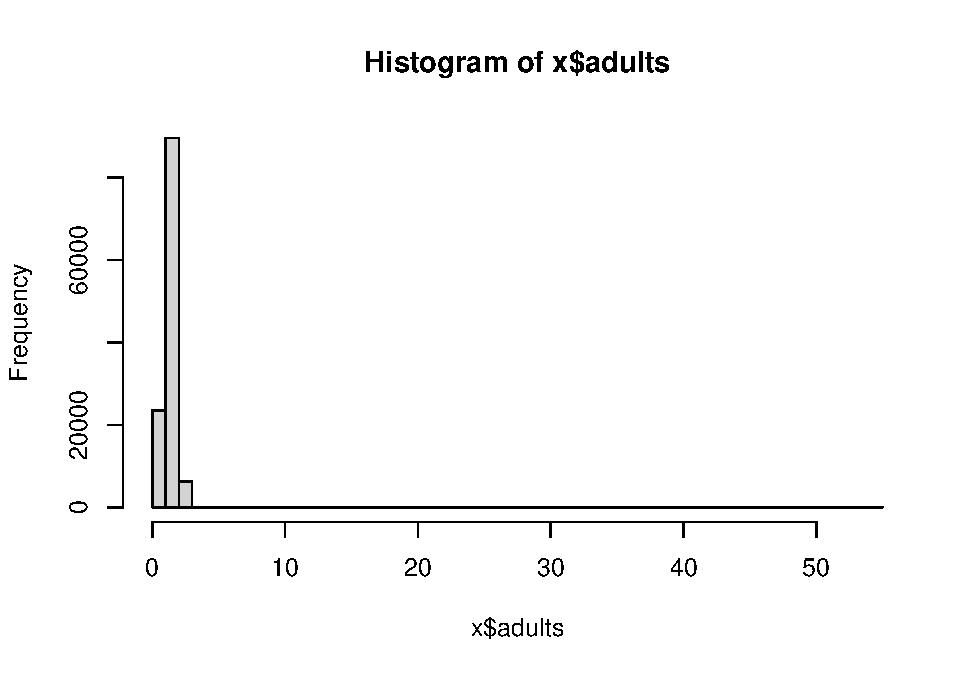
\includegraphics{hotel_bookings_files/figure-latex/hist_adults-1.pdf}

It can be observed that the histogram shows no bars around the value 55,
given that this is a very large set and probably it's only one or a few
cases. In these cases, to analyze the extreme values of a variable, the
values of the variable in question can be represented graphically as
follows, ordering and plotting the data (if they are numerical, as in
this case):

\begin{Shaded}
\begin{Highlighting}[]
\FunctionTok{plot}\NormalTok{(}\FunctionTok{sort}\NormalTok{(x}\SpecialCharTok{$}\NormalTok{adults))}
\FunctionTok{grid}\NormalTok{()}
\end{Highlighting}
\end{Shaded}

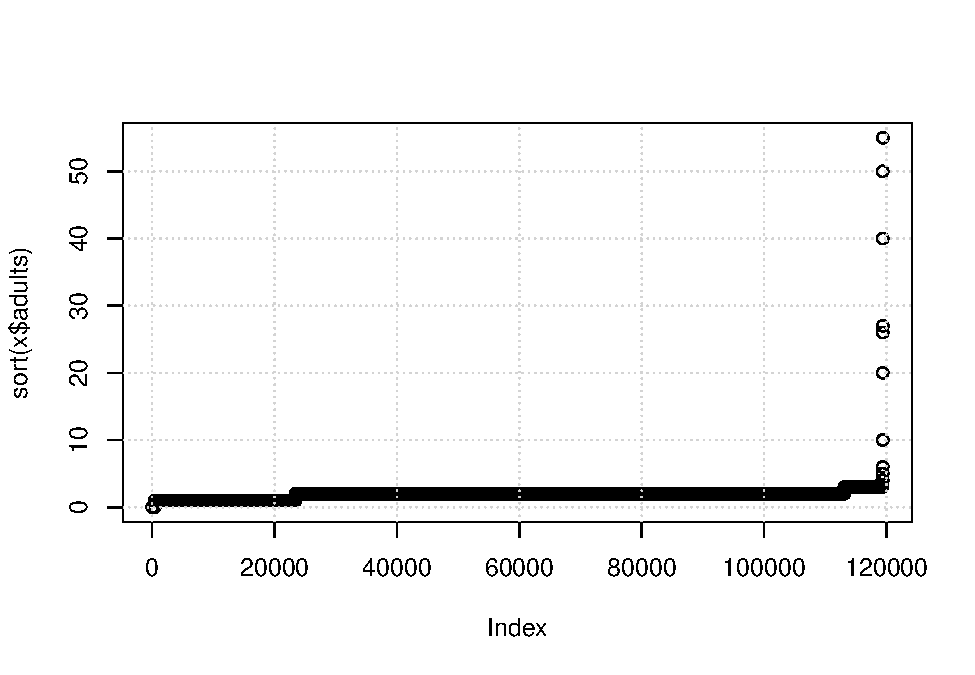
\includegraphics{hotel_bookings_files/figure-latex/plot_adults-1.pdf}
The `Index' represents the position of the element once it's sorted, but
we're more interested in the Y axis, as we can see that some elements
have values of 10 or higher. Since this is an integer variable with a
limited set of possible values, we can use table() to visualize them:

\begin{Shaded}
\begin{Highlighting}[]
\FunctionTok{table}\NormalTok{(x}\SpecialCharTok{$}\NormalTok{adults)}
\end{Highlighting}
\end{Shaded}

\begin{verbatim}
## 
##     0     1     2     3     4     5     6    10    20    26    27    40    50 
##   403 23027 89680  6202    62     2     1     1     2     5     2     1     1 
##    55 
##     1
\end{verbatim}

As you can see, there's one reservation for 10 adults, two for 20
adults, and so on, up to one for 55 adults! Without going into further
detail, we'll remove all rows with reservations for 10 or more adults:

\begin{Shaded}
\begin{Highlighting}[]
\NormalTok{x}\OtherTok{=}\NormalTok{x[x}\SpecialCharTok{$}\NormalTok{adults}\SpecialCharTok{\textless{}}\DecValTok{10}\NormalTok{,]}
\end{Highlighting}
\end{Shaded}

EXERCISE: Repeat this process with variables `children' and `babies'.
Try also to change the threshold to less than 5 instead of 10.

The histogram of the `adr' variable (average daily rate) presents the
same problem as the `adults' variable, so we will simply create a graph
with the ordered values again:

\begin{Shaded}
\begin{Highlighting}[]
\FunctionTok{plot}\NormalTok{(}\FunctionTok{sort}\NormalTok{(x}\SpecialCharTok{$}\NormalTok{adr))}
\FunctionTok{grid}\NormalTok{()}
\end{Highlighting}
\end{Shaded}

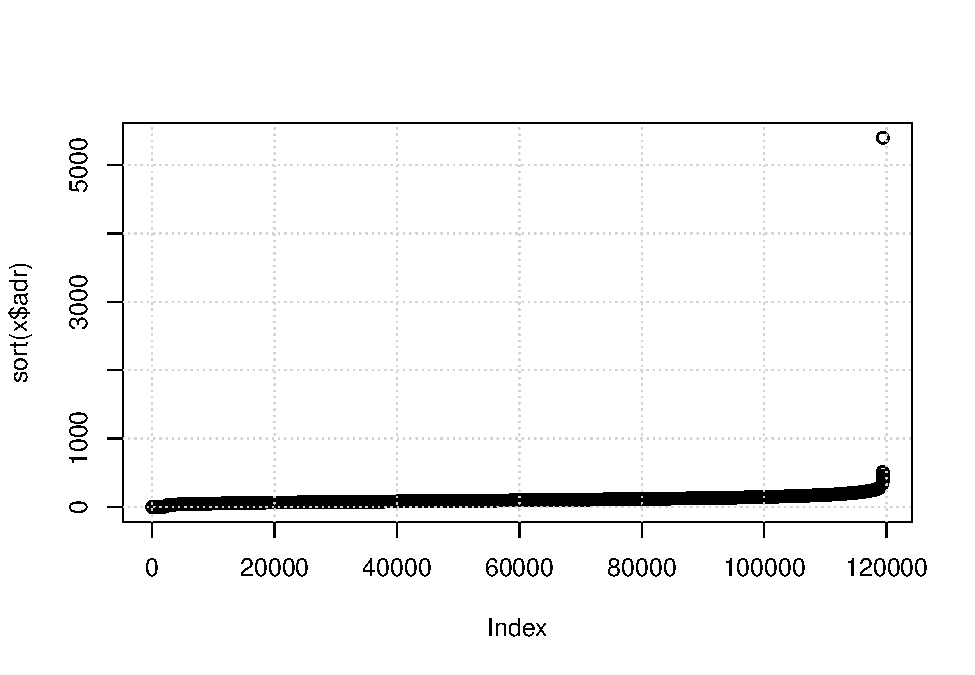
\includegraphics{hotel_bookings_files/figure-latex/plot_adr-1.pdf} In
this case, we observe that only one value is significantly higher than
the rest. We consider it an outlier and eliminate it, as well as the
negative values which have no a clear explanation, although we keep the
0 values:

\begin{Shaded}
\begin{Highlighting}[]
\NormalTok{x}\OtherTok{=}\NormalTok{x[x}\SpecialCharTok{$}\NormalTok{adr}\SpecialCharTok{\textgreater{}=}\DecValTok{0} \SpecialCharTok{\&}\NormalTok{ x}\SpecialCharTok{$}\NormalTok{adr}\SpecialCharTok{\textless{}}\DecValTok{1000}\NormalTok{,]}
\end{Highlighting}
\end{Shaded}

The histogram now provides us with some relevant information. We draw it
using the ggplot2 package, which offers many more options than hist():

\begin{Shaded}
\begin{Highlighting}[]
\FunctionTok{ggplot}\NormalTok{(}\AttributeTok{data=}\NormalTok{x, }\FunctionTok{aes}\NormalTok{(}\AttributeTok{x=}\NormalTok{adr)) }\SpecialCharTok{+} 
  \FunctionTok{geom\_histogram}\NormalTok{(}\AttributeTok{bins=}\DecValTok{55}\NormalTok{, }\AttributeTok{colour=}\StringTok{"black"}\NormalTok{, }\AttributeTok{fill =} \StringTok{"lightgray"}\NormalTok{) }\SpecialCharTok{+}
  \FunctionTok{theme\_light}\NormalTok{()}
\end{Highlighting}
\end{Shaded}

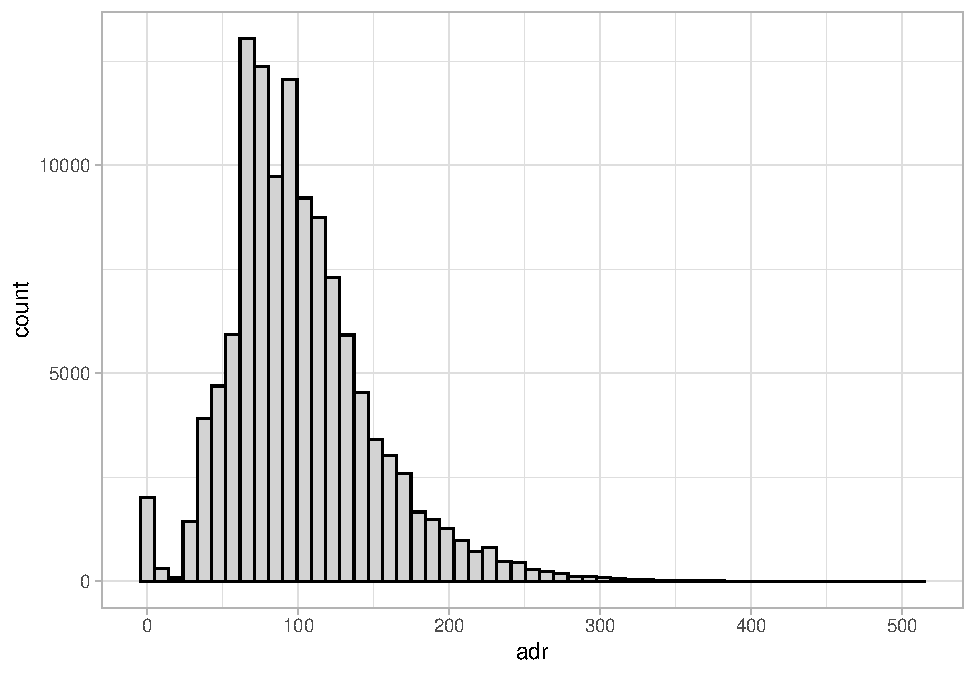
\includegraphics{hotel_bookings_files/figure-latex/hist_adr-1.pdf}
EXERCISE: improve the graph to make axis, title, etc. more adequate.

We can see that there is a set of approximately 2,000 zero values, which
could be analyzed separately, for example. There are R packages that
help us estimate this distribution and the parameters that determine it
visually, such as the fitdistrplus package, which provides the
descdist() function (caution, slow!):

\begin{Shaded}
\begin{Highlighting}[]
\FunctionTok{require}\NormalTok{(fitdistrplus)}
\FunctionTok{descdist}\NormalTok{(x}\SpecialCharTok{$}\NormalTok{adr,}\AttributeTok{boot=}\DecValTok{1000}\NormalTok{)}
\end{Highlighting}
\end{Shaded}

\includegraphics{hotel_bookings_files/figure-latex/descdist-1.pdf}

\begin{verbatim}
## summary statistics
## ------
## min:  0   max:  510 
## median:  94.6 
## mean:  101.7987 
## estimated sd:  48.14364 
## estimated skewness:  1.018857 
## estimated kurtosis:  5.13317
\end{verbatim}

As you can see, the real data (observations, a colored dot) and the
simulated data (in other color) approximate what a lognormal
distribution might look like. However, to experiment with the cleanest
possible data set, we will:

\begin{enumerate}
\def\labelenumi{\arabic{enumi})}
\tightlist
\item
  remove 0-day stays
\item
  remove 0-cost stays
\item
  remove stays with no guests
\item
  replace the NAs in the children variable with 0
\end{enumerate}

\begin{Shaded}
\begin{Highlighting}[]
\NormalTok{x[}\FunctionTok{is.na}\NormalTok{(x}\SpecialCharTok{$}\NormalTok{children),}\StringTok{\textquotesingle{}children\textquotesingle{}}\NormalTok{]}\OtherTok{=}\DecValTok{0}
\NormalTok{x}\OtherTok{=}\NormalTok{x[x}\SpecialCharTok{$}\NormalTok{adr}\SpecialCharTok{\textgreater{}}\DecValTok{0} \SpecialCharTok{\&} 
\NormalTok{    (x}\SpecialCharTok{$}\NormalTok{stays\_in\_week\_nights}\SpecialCharTok{+}\NormalTok{x}\SpecialCharTok{$}\NormalTok{stays\_in\_weekend\_nights)}\SpecialCharTok{\textgreater{}}\DecValTok{0} \SpecialCharTok{\&} 
\NormalTok{    (x}\SpecialCharTok{$}\NormalTok{adults}\SpecialCharTok{+}\NormalTok{x}\SpecialCharTok{$}\NormalTok{children}\SpecialCharTok{+}\NormalTok{x}\SpecialCharTok{$}\NormalTok{babies)}\SpecialCharTok{\textgreater{}}\DecValTok{0} \SpecialCharTok{\&} 
    \SpecialCharTok{!}\FunctionTok{is.na}\NormalTok{(x}\SpecialCharTok{$}\NormalTok{children),]}
\end{Highlighting}
\end{Shaded}

\subsection{Categorical variables}\label{categorical-variables}

For categorical variables, the summary() function gives us a first idea
of the possible values each can take. For example, in the original set
(before removing outliers), there are 79,330 reservations at a city
hotel (Lisbon) and 40,060 at a resort (Algarve). We can ask ourselves
whether the cost distribution is the same for both groups, either by
using the appropriate statistical test or simply by comparing
histograms, in this case using the ggplot2 package, which is much more
powerful for creating all kinds of graphs:

\begin{Shaded}
\begin{Highlighting}[]
\CommentTok{\# require(ggplot2)}
\FunctionTok{ggplot}\NormalTok{(}\AttributeTok{data=}\NormalTok{x, }\FunctionTok{aes}\NormalTok{(}\AttributeTok{x=}\NormalTok{adr, }\AttributeTok{fill=}\NormalTok{hotel)) }\SpecialCharTok{+} 
  \FunctionTok{geom\_histogram}\NormalTok{(}\AttributeTok{bins=}\DecValTok{50}\NormalTok{, }\AttributeTok{colour=}\StringTok{"black"}\NormalTok{) }\SpecialCharTok{+}
  \FunctionTok{theme\_light}\NormalTok{()}
\end{Highlighting}
\end{Shaded}

\includegraphics{hotel_bookings_files/figure-latex/hist_adr_tipo-1.pdf}
It can be seen that the most common prices in Lisbon (city hotels) are
slightly to the right of the most common prices in the Algarve (resort
hotels), although the highest prices in Lisbon decrease more rapidly
than in the Algarve. By using a violin plot, we can see more detail,
especially if we also show the typical quartiles of a box plot:

\begin{Shaded}
\begin{Highlighting}[]
\FunctionTok{ggplot}\NormalTok{(}\AttributeTok{data=}\NormalTok{x, }\FunctionTok{aes}\NormalTok{(}\AttributeTok{x=}\NormalTok{hotel, }\AttributeTok{y=}\NormalTok{adr, }\AttributeTok{fill=}\NormalTok{hotel)) }\SpecialCharTok{+} 
  \FunctionTok{geom\_violin}\NormalTok{() }\SpecialCharTok{+} \FunctionTok{geom\_boxplot}\NormalTok{(}\AttributeTok{width=}\NormalTok{.}\DecValTok{1}\NormalTok{, }\AttributeTok{outliers =}\NormalTok{ F) }\SpecialCharTok{+}
  \FunctionTok{coord\_flip}\NormalTok{() }\SpecialCharTok{+} 
  \FunctionTok{theme\_light}\NormalTok{()}
\end{Highlighting}
\end{Shaded}

\includegraphics{hotel_bookings_files/figure-latex/violin_adr_tipo-1.pdf}
There is an R package called ggstatsplot that has specific functions for
each type of graph, including appropriate statistical tests to determine
if there are differences between groups:

\begin{Shaded}
\begin{Highlighting}[]
\CommentTok{\# require(ggstatsplot)}
\FunctionTok{ggbetweenstats}\NormalTok{(}\AttributeTok{data=}\NormalTok{x, }\AttributeTok{x=}\NormalTok{hotel, }\AttributeTok{y=}\NormalTok{adr)}
\end{Highlighting}
\end{Shaded}

\includegraphics{hotel_bookings_files/figure-latex/ggstatsplot-1.pdf}
Another interesting variable is the hotel guests' origin (`country').
The problem is that this variable has many different values (178), so we
should focus on the countries with the most tourists, also showing
whether they choose a city hotel or a resort:

\begin{Shaded}
\begin{Highlighting}[]
\CommentTok{\# require(tidyverse)}
\CommentTok{\# countries with at least 100 bookings}
\NormalTok{xx }\OtherTok{=}\NormalTok{ x }\SpecialCharTok{\%\textgreater{}\%} \FunctionTok{group\_by}\NormalTok{(country) }\SpecialCharTok{\%\textgreater{}\%} \FunctionTok{mutate}\NormalTok{(}\AttributeTok{pais=}\FunctionTok{n}\NormalTok{()) }\SpecialCharTok{\%\textgreater{}\%} \FunctionTok{filter}\NormalTok{(pais}\SpecialCharTok{\textgreater{}=}\DecValTok{100}\NormalTok{)}
\NormalTok{xx}\SpecialCharTok{$}\NormalTok{country}\OtherTok{=}\FunctionTok{factor}\NormalTok{(xx}\SpecialCharTok{$}\NormalTok{country)}
\FunctionTok{ggplot}\NormalTok{(}\AttributeTok{data=}\NormalTok{xx, }\FunctionTok{aes}\NormalTok{(}\AttributeTok{x=}\FunctionTok{reorder}\NormalTok{(country, }\SpecialCharTok{{-}}\NormalTok{pais))) }\SpecialCharTok{+} 
  \FunctionTok{geom\_bar}\NormalTok{(}\AttributeTok{stat=}\StringTok{"count"}\NormalTok{, }\FunctionTok{aes}\NormalTok{(}\AttributeTok{fill=}\NormalTok{hotel)) }\SpecialCharTok{+}
  \FunctionTok{theme\_light}\NormalTok{() }\SpecialCharTok{+} 
  \FunctionTok{theme}\NormalTok{(}\AttributeTok{axis.text.x =} \FunctionTok{element\_text}\NormalTok{(}\AttributeTok{angle =} \DecValTok{90}\NormalTok{, }\AttributeTok{vjust =} \FloatTok{0.5}\NormalTok{, }\AttributeTok{hjust=}\DecValTok{1}\NormalTok{)) }
\end{Highlighting}
\end{Shaded}

\includegraphics{hotel_bookings_files/figure-latex/country-1.pdf}
Obviously, Portugal (PRT) ranks first, followed by neighboring countries
such as Great Britain, France, and Spain. Visitors from Great Britain
and Ireland are most likely to choose a resort, while those from France,
Germany, and Italy primarily visit Lisbon.

EXERCISE: Are there differences between residents of Portugal and the
rest?

Another interesting variable is `is\_canceled', which indicates whether
a reservation was canceled or not (37.0\% of the time). We can observe
the relationship between two categorical variables using a mosaic chart:

\begin{Shaded}
\begin{Highlighting}[]
\CommentTok{\# require(ggmosaic)}
\NormalTok{x}\SpecialCharTok{$}\NormalTok{is\_canceled}\OtherTok{=}\FunctionTok{as.factor}\NormalTok{(x}\SpecialCharTok{$}\NormalTok{is\_canceled)}
\FunctionTok{ggplot}\NormalTok{(}\AttributeTok{data=}\NormalTok{x) }\SpecialCharTok{+} 
  \FunctionTok{geom\_mosaic}\NormalTok{(}\FunctionTok{aes}\NormalTok{(}\AttributeTok{x=}\FunctionTok{product}\NormalTok{(is\_canceled, hotel), }\AttributeTok{fill=}\NormalTok{hotel)) }\SpecialCharTok{+}
  \FunctionTok{theme\_light}\NormalTok{() }
\end{Highlighting}
\end{Shaded}

\begin{verbatim}
## Warning: The `scale_name` argument of `continuous_scale()` is deprecated as of ggplot2
## 3.5.0.
## This warning is displayed once every 8 hours.
## Call `lifecycle::last_lifecycle_warnings()` to see where this warning was
## generated.
\end{verbatim}

\begin{verbatim}
## Warning: The `trans` argument of `continuous_scale()` is deprecated as of ggplot2 3.5.0.
## i Please use the `transform` argument instead.
## This warning is displayed once every 8 hours.
## Call `lifecycle::last_lifecycle_warnings()` to see where this warning was
## generated.
\end{verbatim}

\begin{verbatim}
## Warning: `unite_()` was deprecated in tidyr 1.2.0.
## i Please use `unite()` instead.
## i The deprecated feature was likely used in the ggmosaic package.
##   Please report the issue at <https://github.com/haleyjeppson/ggmosaic>.
## This warning is displayed once every 8 hours.
## Call `lifecycle::last_lifecycle_warnings()` to see where this warning was
## generated.
\end{verbatim}

\includegraphics{hotel_bookings_files/figure-latex/mosaic_hotel_is_canceled-1.pdf}
It can be seen that the cancellation rate (denoted by 1 on the Y-axis)
at a resort is lower than that of a hotel in Lisbon. On the X-axis, the
relative size of each column also corresponds to the proportion of each
hotel type. It is important not to consider the Y-axis labels (0/1) as
the actual numerical cancellation rate, as this can be misleading.

EXERCISE: which other type of graph could be used to represent this
data?

In the case of cancellation by country for the countries with more
tourists:

\begin{Shaded}
\begin{Highlighting}[]
\CommentTok{\# at least 1000 bookings}
\NormalTok{xx }\OtherTok{=}\NormalTok{ x }\SpecialCharTok{\%\textgreater{}\%} \FunctionTok{group\_by}\NormalTok{(country) }\SpecialCharTok{\%\textgreater{}\%} \FunctionTok{mutate}\NormalTok{(}\AttributeTok{pais=}\FunctionTok{n}\NormalTok{()) }\SpecialCharTok{\%\textgreater{}\%} \FunctionTok{filter}\NormalTok{(pais}\SpecialCharTok{\textgreater{}=}\DecValTok{1000}\NormalTok{)}
\NormalTok{xx}\SpecialCharTok{$}\NormalTok{country}\OtherTok{=}\FunctionTok{factor}\NormalTok{(xx}\SpecialCharTok{$}\NormalTok{country)}
\FunctionTok{ggplot}\NormalTok{(}\AttributeTok{data=}\NormalTok{xx) }\SpecialCharTok{+} 
  \FunctionTok{geom\_mosaic}\NormalTok{(}\FunctionTok{aes}\NormalTok{(}\AttributeTok{x=}\FunctionTok{product}\NormalTok{(is\_canceled, country), }\AttributeTok{fill=}\NormalTok{country)) }\SpecialCharTok{+}
  \FunctionTok{theme\_light}\NormalTok{() }\SpecialCharTok{+}
  \FunctionTok{theme}\NormalTok{(}\AttributeTok{axis.text.x =} \FunctionTok{element\_text}\NormalTok{(}\AttributeTok{angle =} \DecValTok{90}\NormalTok{, }\AttributeTok{vjust =} \FloatTok{0.5}\NormalTok{, }\AttributeTok{hjust=}\DecValTok{1}\NormalTok{)) }
\end{Highlighting}
\end{Shaded}

\includegraphics{hotel_bookings_files/figure-latex/mosaic_country_is_canceled-1.pdf}
It can be seen that the cancellation rate is much higher for local
tourists (from Portugal, PRT), while it is much lower for the rest of
the countries. However, this graph is not easy to read; in this case,
there is no order of either the countries or the percentage of
cancellations.

EXERCISE: Improve the previous graph to make it more understandable and
consider whether it is possible to visualize the relationships between
three or more categorical variables.

Finally, let's analyze the behavior of reservations relative to the
arrival date. First, using the R lubridate package (a marvel for
manipulating date and time data), we'll create a `day' variable to
determine the day of the week the hotel was checked in and analyze how
many reservations there were each day:

\begin{Shaded}
\begin{Highlighting}[]
\CommentTok{\# require(lubridate)}
\NormalTok{x}\SpecialCharTok{$}\NormalTok{dia}\OtherTok{=}\FunctionTok{as\_date}\NormalTok{(}\FunctionTok{paste0}\NormalTok{(x}\SpecialCharTok{$}\NormalTok{arrival\_date\_year,}\StringTok{\textquotesingle{}{-}\textquotesingle{}}\NormalTok{,x}\SpecialCharTok{$}\NormalTok{arrival\_date\_month,}\StringTok{\textquotesingle{}{-}\textquotesingle{}}\NormalTok{,x}\SpecialCharTok{$}\NormalTok{arrival\_date\_day\_of\_month))}
\FunctionTok{ggplot}\NormalTok{(}\AttributeTok{data=}\NormalTok{x,}\FunctionTok{aes}\NormalTok{(}\AttributeTok{x=}\NormalTok{dia,}\AttributeTok{group=}\NormalTok{arrival\_date\_year,}\AttributeTok{color=}\FunctionTok{as.factor}\NormalTok{(arrival\_date\_year))) }\SpecialCharTok{+} 
  \FunctionTok{geom\_bar}\NormalTok{() }\SpecialCharTok{+} \FunctionTok{scale\_color\_manual}\NormalTok{(}\AttributeTok{values=}\FunctionTok{c}\NormalTok{(}\StringTok{"2015"}\OtherTok{=}\StringTok{"red"}\NormalTok{,}\StringTok{"2016"}\OtherTok{=}\StringTok{"green"}\NormalTok{,}\StringTok{"2017"}\OtherTok{=}\StringTok{"blue"}\NormalTok{)) }\SpecialCharTok{+} 
  \FunctionTok{theme\_light}\NormalTok{() }\SpecialCharTok{+} 
  \FunctionTok{theme}\NormalTok{(}\AttributeTok{legend.position=}\StringTok{\textquotesingle{}none\textquotesingle{}}\NormalTok{) }
\end{Highlighting}
\end{Shaded}

\includegraphics{hotel_bookings_files/figure-latex/dia-1.pdf} EXERCISE:
Improve and split the above graph by hotel type or country of origin.

As described in the article, the data covers the period from July 1,
2015, to August 31, 2017. Some peaks can be observed that might be
interesting to explain (what happened those days, i.e.~2015-12-05?). You
can check Google Trends to get some insights:

\url{https://trends.google.es/trends/explore?date=2015-01-01\%202017-12-31&q=lisboa,algarve&hl=es}

\begin{Shaded}
\begin{Highlighting}[]
\FunctionTok{max}\NormalTok{(}\FunctionTok{table}\NormalTok{(x}\SpecialCharTok{$}\NormalTok{dia))}
\end{Highlighting}
\end{Shaded}

\begin{verbatim}
## [1] 439
\end{verbatim}

\begin{Shaded}
\begin{Highlighting}[]
\FunctionTok{which.max}\NormalTok{(}\FunctionTok{table}\NormalTok{(x}\SpecialCharTok{$}\NormalTok{dia))}
\end{Highlighting}
\end{Shaded}

\begin{verbatim}
## 2015-12-05 
##        158
\end{verbatim}

With the computed day `dia', along with the variables `stays\_in\_week'
and `weekend\_nights', we can try to manually categorize the trip type
according to the following criteria (this is arbitrary, clearly
improvable):

\begin{enumerate}
\def\labelenumi{\arabic{enumi})}
\tightlist
\item
  if `stays\_in\_weekend\_nights' is zero =\textgreater{} work trip
\item
  if `stays\_in\_week\_nights' is zero or one and in this case the entry
  is on Friday =\textgreater{} weekend
\item
  if `stays\_in\_week\_nights' is five and `stays\_in\_weekend\_nights'
  is three (that is, from Saturday or Sunday to Saturday or Sunday)
  =\textgreater{} week holiday package
\item
  if `stays\_in\_weekend\_nights' is one or two and
  `stays\_in\_week\_days' is five or less =\textgreater{} work + rest
\item
  the rest of combinations =\textgreater{} holidays
\end{enumerate}

\begin{Shaded}
\begin{Highlighting}[]
\CommentTok{\# require(lubridate)}
\NormalTok{x}\SpecialCharTok{$}\NormalTok{tipo}\OtherTok{=}\FunctionTok{ifelse}\NormalTok{(x}\SpecialCharTok{$}\NormalTok{stays\_in\_weekend\_nights}\SpecialCharTok{==}\DecValTok{0}\NormalTok{, }\StringTok{"work"}\NormalTok{,}
       \FunctionTok{ifelse}\NormalTok{(x}\SpecialCharTok{$}\NormalTok{stays\_in\_week\_nights}\SpecialCharTok{==}\DecValTok{0}\NormalTok{, }\StringTok{"weekend"}\NormalTok{,}
       \FunctionTok{ifelse}\NormalTok{(x}\SpecialCharTok{$}\NormalTok{stays\_in\_week\_nights}\SpecialCharTok{==}\DecValTok{1} \SpecialCharTok{\&} \FunctionTok{wday}\NormalTok{(x}\SpecialCharTok{$}\NormalTok{dia)}\SpecialCharTok{==}\DecValTok{6}\NormalTok{, }\StringTok{"weekend"}\NormalTok{,}
       \FunctionTok{ifelse}\NormalTok{(x}\SpecialCharTok{$}\NormalTok{stays\_in\_week\_nights}\SpecialCharTok{==}\DecValTok{5} \SpecialCharTok{\&} 
\NormalTok{              (x}\SpecialCharTok{$}\NormalTok{stays\_in\_weekend\_nights}\SpecialCharTok{==}\DecValTok{3} \SpecialCharTok{|}
\NormalTok{               x}\SpecialCharTok{$}\NormalTok{stays\_in\_weekend\_nights}\SpecialCharTok{==}\DecValTok{4}\NormalTok{), }\StringTok{"package"}\NormalTok{,}
       \FunctionTok{ifelse}\NormalTok{(x}\SpecialCharTok{$}\NormalTok{stays\_in\_week\_nights}\SpecialCharTok{\textless{}=}\DecValTok{5} \SpecialCharTok{\&} 
\NormalTok{              x}\SpecialCharTok{$}\NormalTok{stays\_in\_weekend\_nights}\SpecialCharTok{\textless{}}\DecValTok{3}\NormalTok{, }\StringTok{"work+rest"}\NormalTok{,}
       \StringTok{"rest"}\NormalTok{)))))}
\end{Highlighting}
\end{Shaded}

One way to refine this classification would be to look at the number of
adults, children, and infants to decide whether it is a business
traveler or a family. The possibilities are endless: you can enrich the
dataset with geographic data (distance between countries), demographic
data, economic data (per capita income), weather data (in both Portugal
and the country of origin), etc.

EXERCISE: You must explore such enriched dataset and, in this process of
exploration, decide what story you want to tell about it. Some ideas:

\begin{enumerate}
\def\labelenumi{\arabic{enumi})}
\tightlist
\item
  do tourists from different countries travel in different dates?
\item
  differences in cancellations among groups (countries, type of stay,
  \ldots)
\item
  relationship between type of stay `tipo' and cost `adr'
\item
  differences among groups with respect to hotel type (city / resort)
\end{enumerate}

NOTE: This is a good example of using ChatGPT or other generative AI to
ask interesting questions about the proposed dataset. The following
paper describes the potential uses of generative AI in the different
phases of creating a data visualization for storytelling:

\url{https://ieeexplore.ieee.org/stamp/stamp.jsp?arnumber=10891192}

\end{document}
